\chapter{前期准备与相关工作}
\section{前期准备}

倒立摆系统的控制,可以采用经典的PID控制方法,LQR控制,模糊控制法,神经网络控制算法,根轨迹控制算法等,我们组搜集了LQR,模糊算法,神经网络算法,以及PID相关方面的资料,进行比较整理,从四种方法中选取了LQR和模糊控制算法进行研究设计。并对研究内容,进度规划,报告,答辩进行了细致的分工,按照计划甘特图推进课程设计,如图~\ref{fig:gant}所示。

\begin{figure}[h]
\centering
    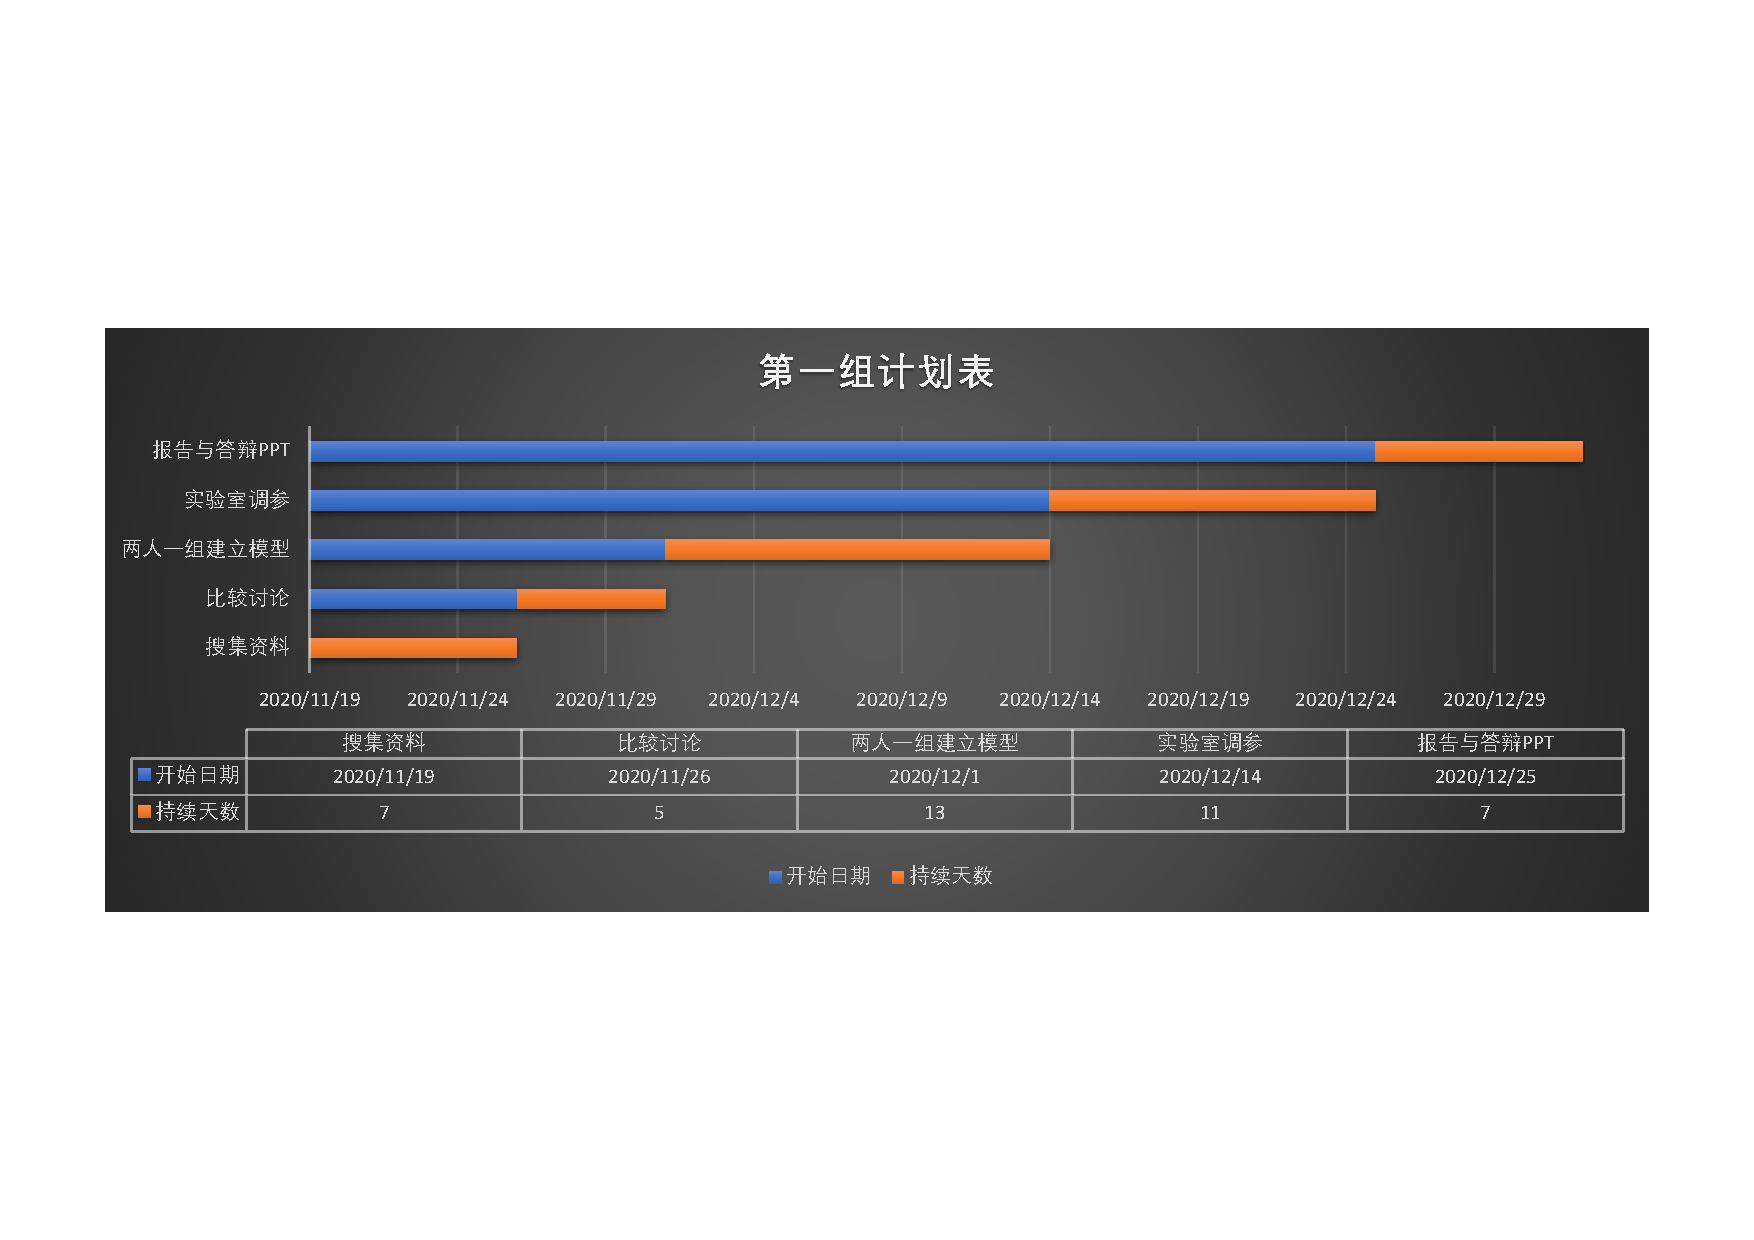
\includegraphics[width=12cm]{gant.pdf}
    \caption{任务计划甘特图}
    \label{fig:gant}
\end{figure}


根据查找的文献资料,我们简单总结了四种控制方法的优缺点,现罗列如下

\subsection{LQR(线性二次型调节器)}
 LQR具有较好的控制住摆杆,并且响应速度较快,具有超调量。该方法可以使目标函数达到最优,可以对能控系统进行任意的极点配置来满足所设计系统的性能要求,提高闭环系统的相对稳定性或者使不稳定系统得以镇定,同时具有较强的鲁棒性。但对小车的控制效果稍差,并且LQR需要调整两个矩阵,要求解$Riccati$方程确定$Q$和$R$权矩阵,算法复杂。

\subsection{模糊控制}
基于模糊控制的方法使用语言方法,可不需要过程的精确数学模型;鲁棒性强,适于解决过程控制中的非线性、强耦合时变、滞后等问题;
有较强的容错能力。具有适应受控对象动力学特征变化、环境特征变化和动行条件变化的能力。但是模糊控制的设计尚缺乏系统性,这对复杂系统的控制是难以奏效的。难以建立一套系统的模糊控制理论,以解决模糊控制的机理、稳定性分析、系统化设计方法等一系列问题;如何获得模糊规则及隶属函数即系统的设计办法,完全凭经验进行;信息简单的模糊处理将导致系统的控制精度降低和动态品质变差。若要提高精度就必然增加量化级数,导致规则搜索范围扩大,降低决策速度,甚至不能进行实时控制。

\subsection{神经网络}
基于神经网络的算法属于非线性映射,能以任意精度逼近任何非线性连续函数,适合求解内部机制复杂问题。
而且输入输出变量数目是任意的,具有自学习和自适应的能力,能过学习获取输出数据间的对应关系,将学习内容存储到网络权值中,具有容错能力,部分神经元受损对全局训练结果不会有很大影响。但是该方法存在实时性和自适应性相互矛盾的问题,不能保证快速性和有效性;并且权值容易收敛到局部最小点,收敛速度慢,隐含层数目难以确定,训练依赖样本数据,样本数据有采集难度。

\subsection{PID控制}
基于PID原理的控制系统结构简单,易于实现,使用方便,PID各参数相互独立,可以根据过程的动态特性及时调节;
适用性强,可通过适当简化将非线性的、时变的被控对象变成基本线性和动态特性不随时间变化的系统,应用范围十分广泛,理论成熟。
棒性较好,即其控制品质对被控对象特性的变化不太敏感。
但是该方法稳定性差,在控制非线性、时变、耦合及参数和结构不确定的复杂过程时,效果不好。

\section{题目数据}

将题目的数据整理如表~\ref{para}所示。

\begin{table}[h]
\centering
\begin{tabular}{ccc}
\hline
参数 & 意义           & 数值                            \\ \hline
$M$  & 小车质量         & $1.096kg$                       \\ \hline
$m$ & 摆杆质量         & $0.109kg$                       \\ \hline
$l$  & 摆杆质心到转动轴心的长度 & $0.25m$                         \\ \hline
$b$  & 摩擦比例系数       & $0.1N.s/m$                      \\ \hline
$I$  & 摆杆对质心的转动惯量   & $0.0034kg.m^2$ \\ \hline
$T$  & 采样时间         & $0.005s$                        \\ \hline
\end{tabular}
\caption{题目参数}\label{para}
\end{table}

\chapter{物理模型的建立和状态空间公式的推导}

为了建立物理模型,现有如下假设:

1、摆杆质量均匀,质心位于其几何中心处

2、忽略除b以外的所有摩擦力


如图\ref{fig:car}对小车进行受力分析,以摆杆和小车交点为原点,以水平向右和竖直向下为正方向建立坐标系,沿$x$轴有牛顿第二定律

\begin{figure}[hbpt]
\centering
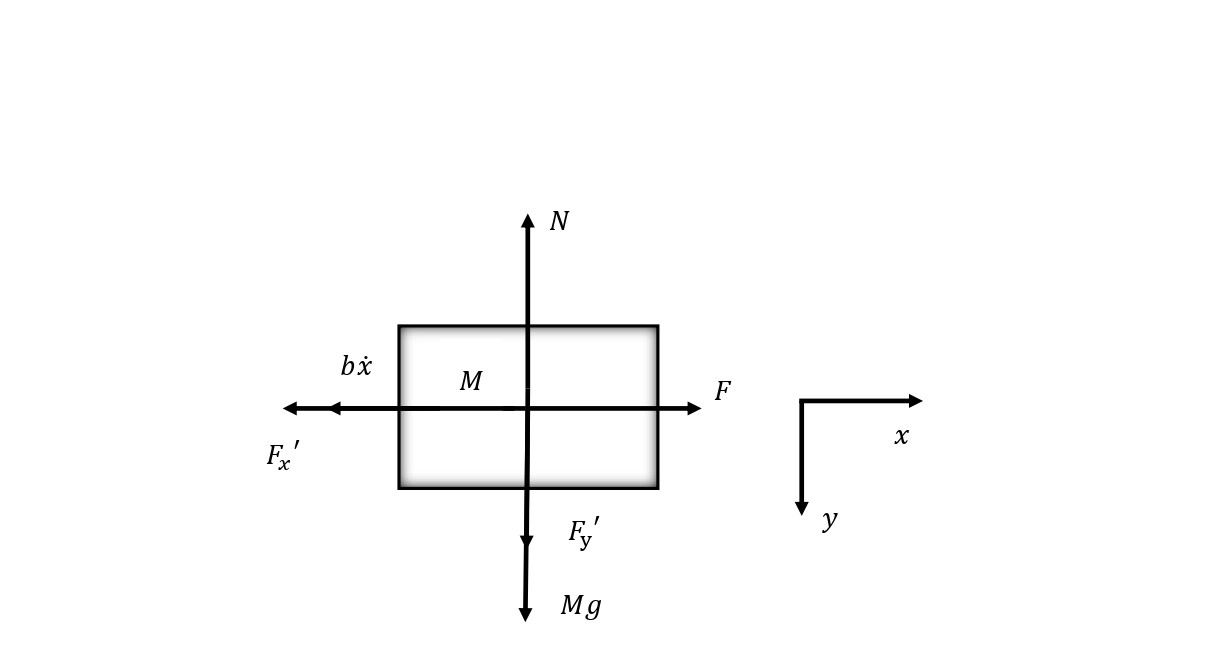
\includegraphics[width=12cm]{car.jpg}
\caption{小车受力分析}\label{fig:car}
\end{figure}


\begin{equation}
F-b\dot x-N_x^{'}=M\ddot x
\end{equation}

如图\ref{fig:stick}对摆杆进行受力分析,沿$x,y$轴有牛顿第二定律和沿$\theta$向动量矩定理

\begin{figure}[hbpt]
\centering
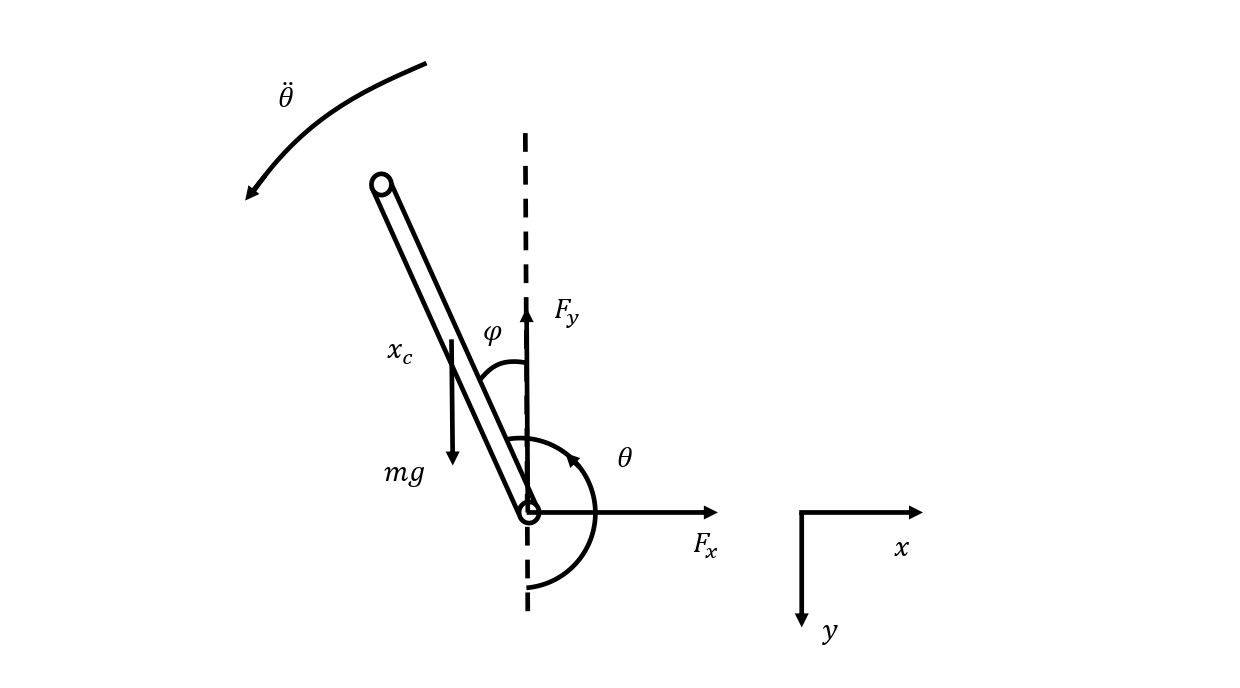
\includegraphics[width=12cm]{stick.jpg}
\caption{摆杆受力分析}\label{fig:stick}
\end{figure}

摆杆质心$c$点
	
\begin{equation}
\begin{aligned}
x_c&=x+lsin\theta\\
y_c&=lcos\theta\\
\end{aligned}
\end{equation}

求导可得质心加速度

\begin{equation}
\begin{aligned}
\ddot x_c&=\ddot x+l\ddot{\theta}cos\theta-l\dot{\theta}^2sin\theta\\
\ddot y_c&=-l\ddot{\theta}sin\theta-l\dot{\theta}^2cos\theta\\
\end{aligned}
\end{equation}
\begin{equation}
\begin{aligned}
&N_y-mg=-m\ddot y_c\\
&N_x=m\ddot x_c\\
&N_ylsin\varphi+N_xlcos\varphi=I\ddot{\varphi}\\
\end{aligned}
\end{equation}

应用小量近似$sinx\doteq x$,$cosx=1-\frac{x^2}{2}$以及$\theta=\varphi+\pi$这个关系整理以上各式,可得倒立摆系统物理方程组

\begin{equation}
\begin{aligned}
&F=(M+m)\ddot x-ml\ddot{\varphi}+b\dot x\\
&(I+ml^2)\ddot{\varphi}=ml\ddot x+mgl\varphi\\
\end{aligned}
\end{equation}

拉氏变换可得

\begin{equation}
\begin{aligned}
&(M+m)X(s)s^2+bX(s)s-ml\varphi(s)s^2=F(s)\\
&(I+ml^2)\varphi(s)s^2-mgl\varphi((s)=mlX(s)s^2\\
\end{aligned}
\end{equation}

注意到小车加速度$A(s)=X(s)s^2$

可得从小车角速度输入到摆杆角度输出的传递函数

\begin{equation}
\frac{\varphi(s)}{A(s)}=\frac{ml}{(I+ml^2)s^2-mgl}
\end{equation}

进一步整理,可以得到力输入到摆杆角度和小车位移的传递函数

\begin{equation}
\begin{aligned}
&\frac{\varphi(s)}{F(s)}=\frac{mls^2}{[(I+ml^2)(M+m)-m^2l^2]s^4+b(I+ml^2)s^3-(M+m)mgls^2-bmgls}\\
&\frac{X(s)}{F(s)}=\frac{(I+ml^2)s^2-mgl}{[(I+ml^2)(M+m)-m^2l^2]s^4+b(I+ml^2)s^3-(M+m)mgls^2-bmgls}
\end{aligned}
\end{equation}

将物理方程组进行等价变形,可以得到

\begin{equation}
\begin{aligned}
&\ddot x=-\frac{bI+bml^2}{\Delta}\dot x+\frac{m^2gl^2}{\Delta}\varphi+\frac{I+ml^2}{\Delta}F\\
&\ddot{\varphi}=\frac{-mlb}{\Delta}\dot x+\frac{mg(M+m)l}{\Delta}\varphi+\frac{ml}{\Delta}F\\
\end{aligned}
\end{equation}

其中,$\Delta=I(M+m)+Mml^2$.

基于此,取$z_1=x,z_2=\dot x,z_3=\varphi,z_4=\dot{\varphi}$为状态空间变量,以力$F$作为输入$u$,建立状态空间矩阵

\begin{equation}
\begin{aligned}
&\begin{bmatrix}
\dot x\\
\ddot x\\
\dot{\varphi}\\
\ddot{\varphi}\\
\end{bmatrix}
=
\begin{bmatrix}
0 & 1 & 0 & 0\\
0 & -\frac{bI+bml^2}{\Delta} & \frac{m^2gl^2}{\Delta} & 0\\
0 & 0 & 0 & 1\\
0 & \frac{-mlb}{\Delta} & \frac{mg(M+m)l}{\Delta} & 0\\
\end{bmatrix}
\begin{bmatrix}
x\\
\dot x\\
\varphi\\
\dot{\varphi}\\
\end{bmatrix}
+
\begin{bmatrix}
0\\
\frac{I+ml^2}{\Delta}\\
0\\
\frac{ml}{\Delta}\\
\end{bmatrix}
u\\
&\begin{bmatrix}
x\\
\varphi\\
\end{bmatrix}
=
\begin{bmatrix}
1 &0 &0 &0\\
0 &0 &1 &0\\
\end{bmatrix}
\begin{bmatrix}
x\\
\dot x\\
\varphi\\
\dot{\varphi}\\
\end{bmatrix}
+
\begin{bmatrix}
0\\
0\\
\end{bmatrix}
u\\
\end{aligned}
\end{equation}

注意到该状态空间矩阵较为复杂,若取小车加速度作为输入$u^{'}$,可以简化该状态空间矩阵

根据转动惯量的定义式,并认为摆件质地均匀,有下式

\begin{equation}
I=\frac{1}{12}m(2l)^2
\end{equation}

带入整理,得

\begin{equation}
\ddot \varphi=\frac{3g}{4l}\phi+\frac{3}{4l}\ddot x
\end{equation}

则可得较为简单的状态空间矩阵

\begin{equation}
\begin{aligned}
&\begin{bmatrix}
\dot x\\
\ddot x\\
\dot{\varphi}\\
\ddot{\varphi}\\
\end{bmatrix}
=
\begin{bmatrix}
0 & 1 & 0 & 0\\
0 & 0 & 0 & 0\\
0 & 0 & 0 & 1\\
0 & 0 & \frac{3g}{4l} & 0\\
\end{bmatrix}
\begin{bmatrix}
x\\
\dot x\\
\varphi\\
\dot{\varphi}\\
\end{bmatrix}
+
\begin{bmatrix}
0\\
1\\
0\\
\frac{3}{4l}\\
\end{bmatrix}
u'\\
&\begin{bmatrix}
x\\
\varphi\\
\end{bmatrix}
=
\begin{bmatrix}
1 &0 &0 &0\\
0 &0 &1 &0\\
\end{bmatrix}
\begin{bmatrix}
x\\
\dot x\\
\varphi\\
\dot{\varphi}\\
\end{bmatrix}
+
\begin{bmatrix}
0\\
0\\
\end{bmatrix}
u^{'}\\
\end{aligned}
\end{equation}

代入数据可得

\begin{equation}
\begin{aligned}
&\begin{bmatrix}
\dot x\\
\ddot x\\
\dot{\varphi}\\
\ddot{\varphi}\\
\end{bmatrix}
=
\begin{bmatrix}
0 & 1 & 0 & 0\\
0 & 0 & 0 & 0\\
0 & 0 & 0 & 1\\
0 & 0 & 29.4 & 0\\
\end{bmatrix}
\begin{bmatrix}
x\\
\dot x\\
\varphi\\
\dot{\varphi}\\
\end{bmatrix}
+
\begin{bmatrix}
0\\
1\\
0\\
3\\
\end{bmatrix}
u'\\
&\begin{bmatrix}
x\\
\varphi\\
\end{bmatrix}
=
\begin{bmatrix}
1 &0 &0 &0\\
0 &0 &1 &0\\
\end{bmatrix}
\begin{bmatrix}
x\\
\dot x\\
\varphi\\
\dot{\varphi}\\
\end{bmatrix}
+
\begin{bmatrix}
0\\
0\\
\end{bmatrix}
u^{'}\\
\end{aligned}
\end{equation}

\chapter{用PID算法校正直线一级倒立摆系统}
%-------------------------------------------------------------------
\section{PID控制分析}

\subsection{PID介绍}

PID控制就是用线性组合的方式,把偏差的比例$P$、积分$I$、微分$D$组合构成控制量。对被控对象展开控制的方法。在PID控制器中,通过比例单元$P$将偏差进行比例放大得到输出,但通过这一过程无法消除余差,因此加以积分单元$I$,积分依照偏差累计,只要当偏差不为0时,积分值就不为0,考虑到偏差变化有速度快慢之分,加以微分单元$D$,计算偏差变化的速率,PID控制就是综合使用这三个单元来控制被控变量。其原理控制示意图如图~\ref{fig:PID_principle}所示。

\subsection{PID控制器原理性推导}
	
PID控制器是一种线性控制器,其根据给定值$r(t)$与实际输出值$y(t)$构成的控制偏差$e(t)$为:

\begin{figure}[hbpt]
\centering
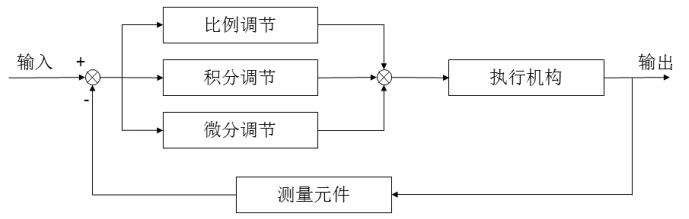
\includegraphics[width=12cm]{PID_principle.png}
\caption{PID原理图}\label{fig:PID_principle}
\end{figure}

\begin{equation}
e(t)=r(t)-y(t)
\end{equation}

其输入控制偏差$e(t)$与输出控制结果$u(t)$的关系为:

\begin{equation}
u(t)=K_pe(t)+K_I\int_0^te(t)dt+K_D \frac{de(t)}{dt}
\end{equation}

上式进行拉氏变换,得其传递函数为:

\begin{equation}
\begin{aligned}
G(s)&=\frac{U(s)}{E(s)}\\
&=K_p+\frac{1}{K_Is}+K_Ds\\
&=\frac{K(\tau_1s+1)(\tau_2s+1)}{s}
\end{aligned}
\end{equation}

其中,$K_pe(t)$为比例环节,随着$K_p$的增加,可以更好地减小偏差,但同时$K_p$还影响系统的稳定性,$K_p$增加通常导致系统的稳定性下降,过大的$K_p$往往使系统产生剧烈的震荡和不稳定。

$K_I\int_0^te(t)dt$为积分环节,消除系统静态误差,作用的强弱由$K_I$决定,$K_I$越大,积分作用越强,反之则越弱,但同时积分环节也可能增大系统超调量。

$K_D\frac{de(t)}{dt}$为微分环节,针对被测量的变化速率来进行调节,预测偏差信号的变化趋势,在其出现较大变化之前引入修正信号与之低效,从而减小系统的调节时间。

\subsection{实验分析}

实验室倒立摆控制系统结构图如图~\ref{fig:structure}所示。

\begin{figure}[hbpt]
\centering
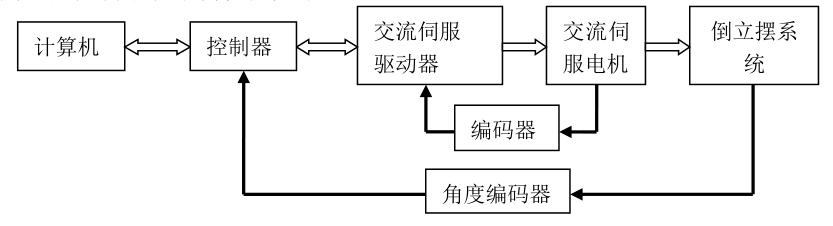
\includegraphics[width=12cm]{structure.png}
\caption{实验室倒立摆控制系统结构图}\label{fig:structure}
\end{figure}

修改PID各项参数,通过角度编码器测量摆杆的摆动角度,通过伺服电机控制小车的位移速度和加速度,通过控制器利用摆杆的惯性力控制摆杆的位移速度和加速度,从而控制摆杆的角度,最终可以实现直线倒立摆的竖直稳定.

当其受到外界干扰时,在干扰停止作用后,系统能够很快地回到平衡位置。但是,整个控制系统中并无小车位移的反馈,只能通过角度编码器获取摆杆的角度,通过传动比转换近似得到小车的位移。因此 PID控制器无法对小车的位置偏差进行修正,不能对小车的位置进行控制,当受到扰动时,小车会沿滑轨一直向扰动方向运动,撞到滑轨边缘,无法恢复到初始平衡位置。后续考虑使用其它控制方法,既能实现直线倒立摆的竖直稳定,又可以控制小车位置的稳定不变。

\chapter{LQR}
\section{LQR线性二次型调节器}

\subsection{LQR介绍}

LQR(linear quadratic regulator)线性二次型调节器,利用现代控制理论中以状态空间矩阵形式给出的线性系统,利用目标函数(能量函数)$J=\frac{1}{2}\int_0^\infty(x^TQx+u^TRu)dt$(其中Q为半正定矩阵,R为正定矩阵),设计状态反馈控制器$K$使得目标函数的值最小。
LQR控制器可以在系统偏离平衡状态时,尽可能减少消耗的能量保持系统状态各分量仍接近平衡状态.以一维系统$X=x(t)$为例,则$x^TQx=Qx^2$,为了使得$J$最小,那么该函数一定有界,故有下式

\begin{equation}
\lim_{t \rightarrow \infty}x(t)=0
\end{equation}

这保证了系统的稳定性,类似的$u(t)$小保证了节省能量,控制代价降低。

\subsection{LQR控制器原理性推导}

线性系统的状态空间可以描述为
	
\begin{equation}
\begin{aligned}
\dot X=AX+Bu\\
Y=CX+Du\\
\end{aligned}
\end{equation}

评价函数为

\begin{equation}
J=\frac{1}{2}\int_0^\infty(x^TQx+u^TRu)dt
\end{equation}

$Q、R$分别是对状态变量和输入量的加权矩阵,确定误差和能量损耗的相对性。

根据极小值原理,引入$n$维协态矢量$\lambda(t)$,构造哈密顿函数

\begin{equation}
H(x,u,\lambda)=\frac{1}{2}[x^TQx+u^TRu]+\lambda^T[Ax+Bu]
\end{equation}

最优控制使得$H$取极值,即

\begin{equation}
\frac{\partial H}{\partial u}=Ru+B^T\lambda=0
\end{equation}

解得

\begin{equation}
u=-R^{-1}B^T\lambda
\end{equation}

又有

\begin{equation}
\frac{\partial^2 H}{\partial u^2}=R
\end{equation}

R正定,故上式为系统的最优控制律。

设$\lambda=Px$,$P$为$n$阶实对称正定矩阵,且满足黎卡提矩阵代数方程

\begin{equation}
-PA-A^TP+PBR^{-1}B^T-Q_1=0
\end{equation}

则最优控制

\begin{equation}
u=-R^{-1}B^T\lambda=-Kx
\end{equation}

系统最优轨线为

\begin{equation}
\dot x(t)=(A-BK)x(t)
\end{equation}

在$matlab$中可以利用$lqr$函数求得反馈矩阵$K$.

\subsection{$LQR$的系统能控性和能观性分析}

对于上面假设的线性系统,状态完全能控制的充要条件是

\begin{equation}
rank[B,AB,A^2B,\dots A^{n-1}B]=n
\end{equation}

系统状态能够完全观测的充要条件是

\begin{equation}
rank
\begin{bmatrix}
C\\
CA\\
CA^2\\
\vdots\\
CA^{n-1}\\
\end{bmatrix}
=n
\end{equation}

\subsection{小车系统权重的选取以及能控性能观性分析}

前面得到小车的状态空间方程为

\begin{equation}
\begin{aligned}
&\begin{bmatrix}
\dot x\\
\ddot x\\
\dot{\varphi}\\
\ddot{\varphi}\\
\end{bmatrix}
=
\begin{bmatrix}
0 & 1 & 0 & 0\\
0 & 0 & 0 & 0\\
0 & 0 & 0 & 1\\
0 & 0 & 29.4 & 0\\
\end{bmatrix}
\begin{bmatrix}
x\\
\dot x\\
\varphi\\
\dot{\varphi}\\
\end{bmatrix}
+
\begin{bmatrix}
0\\
1\\
0\\
3\\
\end{bmatrix}
u'\\
&\begin{bmatrix}
x\\
\varphi\\
\end{bmatrix}
=
\begin{bmatrix}
1 &0 &0 &0\\
0 &0 &1 &0\\
\end{bmatrix}
\begin{bmatrix}
x\\
\dot x\\
\varphi\\
\dot{\varphi}\\
\end{bmatrix}
+
\begin{bmatrix}
0\\
0\\
\end{bmatrix}
u^{'}\\
\end{aligned}
\end{equation}

在$matlab$中(代码见附录)进行矩阵秩计算可知两个判定矩阵的秩都是$4$,则小车倒立摆系统可控可观测。

\subsection{小车倒立摆仿真}

首先根据系统的运动微分方程在$matlab$中的$simulink$进行仿真,由上述矩阵导出参考方程,为方便,将一些量名称更改如下

\begin{equation}
\begin{aligned}
&\dot x\rightarrow \dot x_1\\
&\ddot x\rightarrow \dot x_2\\
&\dot \varphi \rightarrow \dot x_3\\
&\ddot \varphi \rightarrow \dot x_4\\
\end{aligned}
\end{equation}

则有

\begin{equation}
\begin{aligned}
&\dot x_1=x_2\\
&\dot x_2=u\\
&\dot x_3=x_4\\
&\dot x_4=29.4x_3+3u\\
&u=-k_1x_1-k_2x_2-k_3x_3-k_4x_4\\
\end{aligned}
\end{equation}

得到如图~\ref{LQR_simulink}的仿真

\begin{figure}[hbpt]
\centering
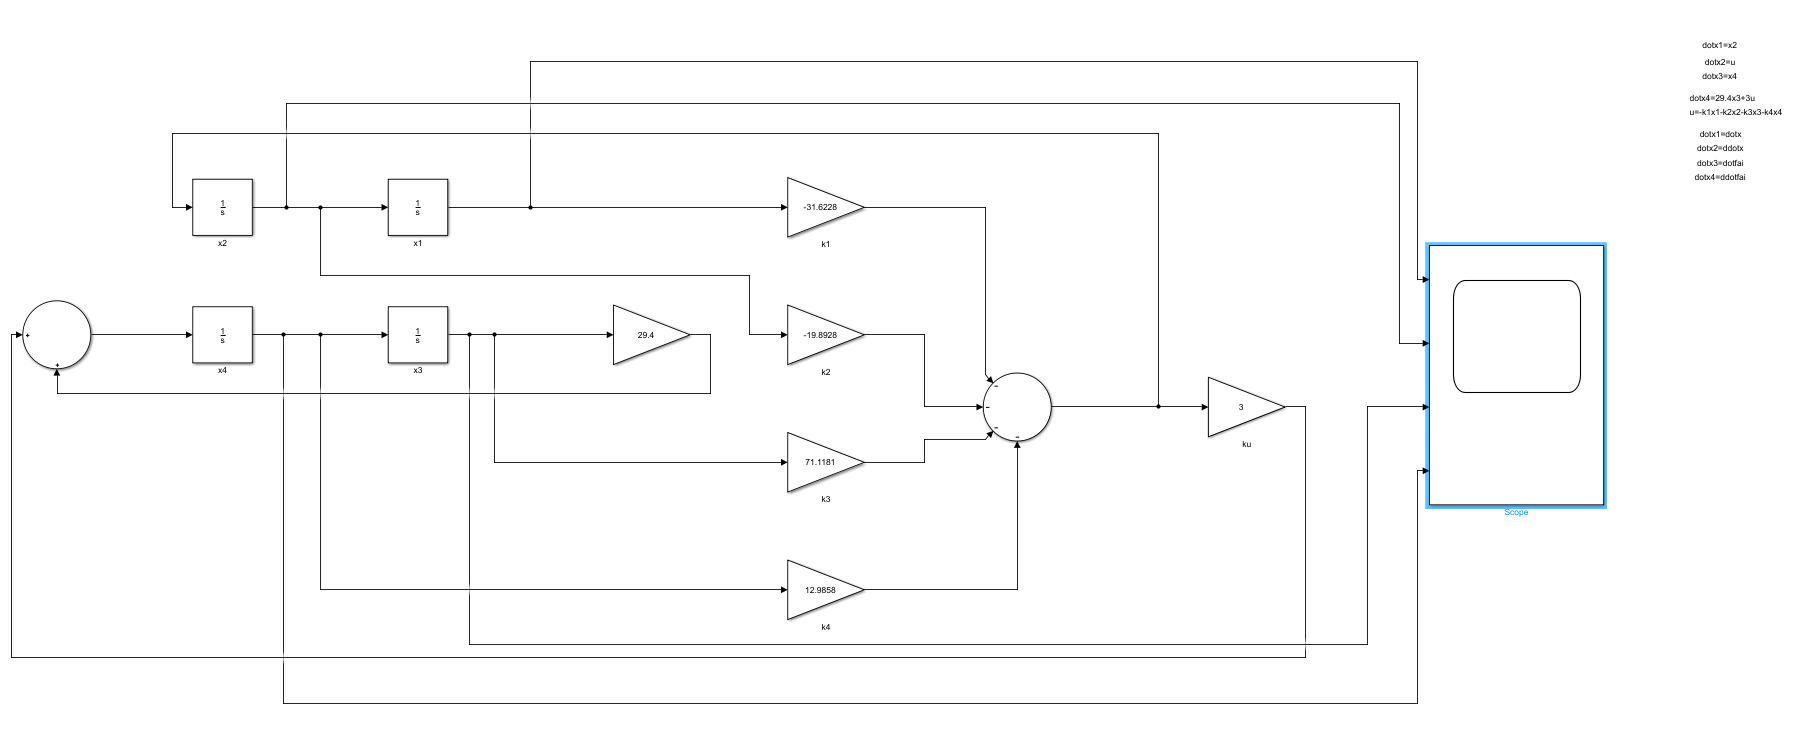
\includegraphics[width=16cm]{LQR_simulink.png}
\caption{$LQR的simulink$}\label{LQR_simulink}
\end{figure}

这种仿真可以通过给定$x_i$的初始值来模拟脉冲激励

\begin{figure}[hbpt]
\centering
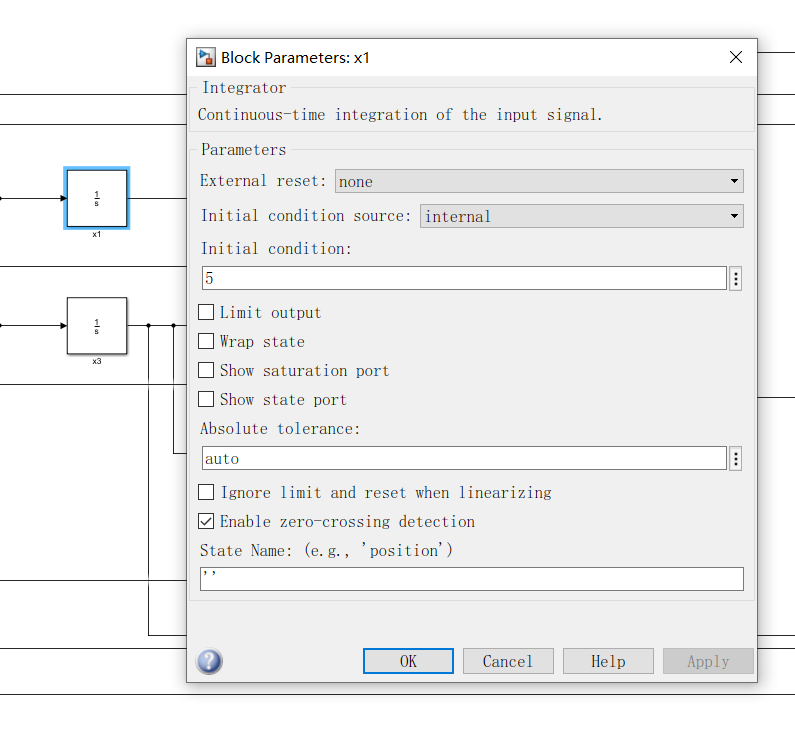
\includegraphics[width=12cm]{initial.png}
\caption{模拟脉冲激励}\label{initial}
\end{figure}

给定小车$5$单位位移,摆杆$5$单位角度,可以得到如图\ref{1000_100}的响应曲线。

\begin{figure}[hbpt]
\centering
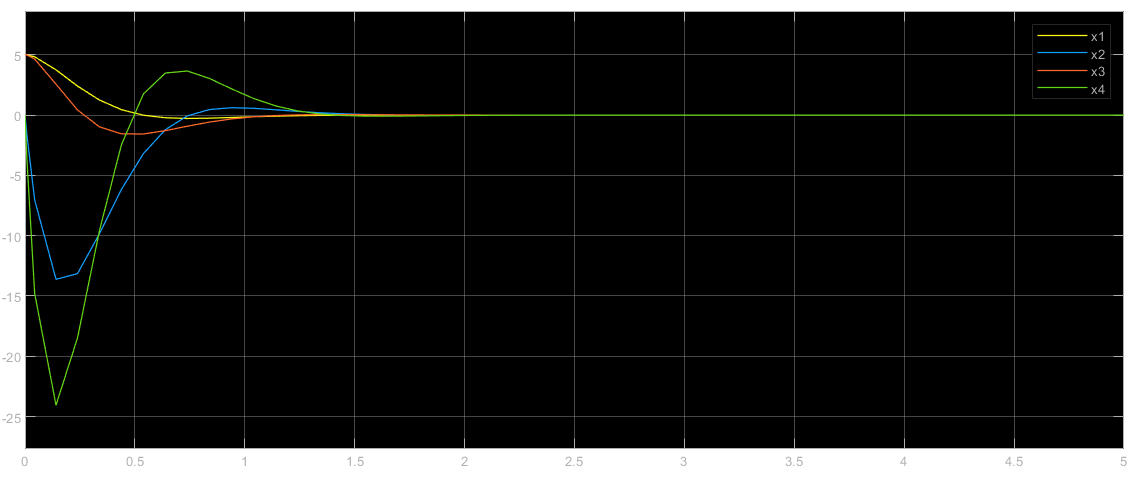
\includegraphics[width=15cm]{1000_100.png}
\caption{脉冲激励仿真结果}\label{1000_100}
\end{figure}

可以发现系统可以稳定。关于修改权重以及关于曲线的比较分析在后面介绍。

此外也可以利用编程来模拟仿真,以$lsim$函数模拟的阶跃信号为例,编写代码(见附件)也可以得到响应曲线如图\ref{1000_100_2}。

\begin{figure}[hbpt]
\centering
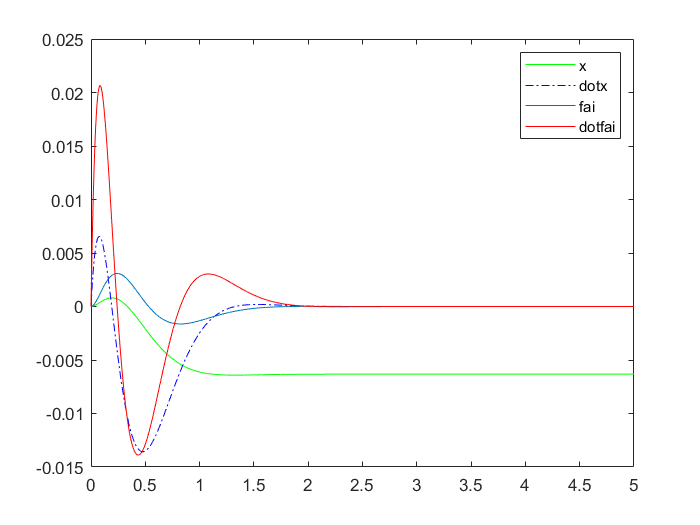
\includegraphics[width=12cm]{1000_100_2.png}
\caption{阶跃激励仿真结果}\label{1000_100_2}
\end{figure}

\subsection{修改权重分析比较}


\newpage
%-----------------------------------------------------
	\appendix
	\ctexset{section={
		format={\zihao{-4}\heiti\raggedright}
	}}
	\begin{center}
		\heiti\zihao{4} 附\hspace{1pc}录
	\end{center}

\begin{lstlisting}
A=[0 1 0 0;
   0 0 0 0;
   0 0 0 1;
   0 0 29.4 0];
B=[0 1 0 3]';
C=[1 0 0 0;
   0 0 0 1];
D=[0 0]';
Co=ctrb(A,B);
rank(Co)
Ob=obsv(A,C);
rank(Ob)
\end{lstlisting}

\begin{lstlisting}
A=[0 1 0 0;0 0 0 0;0 0 0 1;0 0 29.4 0];
B=[0 1 0 3]';
C=[1 0 0 0;0 0 1 0];
D=[0 0 ]';
Q11=1000;
Q33=100;
Q=[Q11 0 0 0;0 0 0 0;0 0 Q33 0;0 0 0 0];
R=1;
K=lqr(A,B,Q,R);
Ac=(A-B*K);
T=0:0.001:5;
U=0.2*ones(size(T));
[Y,X]=lsim(Ac,B,C,D,U,T);
plot(T,X(:,1),'-g','LineWidth',1);
hold on;
plot(T,X(:,2),'-.b','LineWidth',1);
plot(T,X(:,3),'-','LineWidth',1);
plot(T,X(:,4),'-r','LineWidth',1);
hold off;
legend('x','dotx','fai','dotfai');
\end{lstlisting}
